\documentclass[a5paper]{article}

\pagestyle{empty}
\usepackage[ left=3cm
           , right=1cm
           , top=2cm
           , bottom=2cm
           ]{geometry}
\setlength{\parindent}{0ex}
\usepackage{tikz}
\usepackage{calc}
\usepackage{fontspec}

\usepackage{amssymb,pifont,bm}
\newcommand{\cmark}{\ding{51}}%
\newcommand{\xmark}{\ding{55}}%
\newcommand{\memo}{\ding{115}}%
\newcommand{\up}{\ding{216}}

\newcommand{\legend}[1][\footnotesize]{
  #1\color{gray!60}
  \begin{tabular}{rl}
    $\circ$ & event \\
    $\bullet$ & task \\
    \xmark & done\\
    $\boldsymbol{!}$ & impor\\
    \memo & memo\\
    \up & postpone
    \end{tabular}
}

\setmainfont{Liberation Sans}
\newfontfamily{\weekFont}{Liberation Sans}

\makeatletter
  \def\@week#1{%
    \color{gray!45}%
    \fontsize{15}{15}%
    \selectfont%
    \weekFont{#1}
  }
  \def\sunday{\@week{Su}}
  \def\monday{\@week{Mo}}
  \def\tuesday{\@week{Tu}}
  \def\wednesday{\@week{We}}
  \def\thursday{\@week{Th}}
  \def\friday{\@week{Fr}}
  \def\saturday{\@week{Sa}}
\makeatother

\newcommand{\fsize}[1]{\fontsize{#1}{#1}\selectfont}

\def\EOFmonth{31}
\newcommand{\deflength}[2]{\newlength{#1}\setlength{#1}{#2}}
  \deflength{\WW}{\textwidth  - 2mm}
  \deflength{\HH}{\textheight - 2mm}
  \deflength{\WWh}{0.5 \WW}
  \deflength{\HHh}{0.5 \WW}
  \deflength{\trackerSpace}{\HH / \EOFmonth}
  \deflength{\dotSpacing}{\HH / 25}
  \deflength{\spacin}{\HH / \EOFmonth}

\begin{document}


\begin{tikzpicture}
	\draw[white] (0,0) rectangle (\WW,\HH)
	node[black,pos=.5]
		{\fsize{55} ASBJ}
	node[gray!75,pos=.4]
		{\fsize{25} A Simple Bullet Journal};
\end{tikzpicture}

%==[ splash month ]=====================================================
\foreach \month/\len in
	{ January/31
		, February/29
		, March/31
		, April/30
		, May/31
		, June/30
		, July/31
		, August/31
		, September/30
		, October/31
		, November/30
		, December/31
	}{
		\begin{tikzpicture}[yscale=-1]
			\fill[gray!15] (0,0) rectangle (\WW/4,.75\HH)
			node[gray!40,pos=.5] {\rotatebox{90}{\fsize{45} \month}};
			\node[below left] at (\WW/4,0) {\legend};
			\draw[line width=1pt] (\WW,0) -- (0,0) |- (\WW,0.75\HH);
			\foreach \i in {1,...,4}
			\draw[gray!40,ultra thin] (\WW/4,\i * 0.75\HH / 5) -- (\WW,\i * 0.75\HH / 5);
			\foreach \j/\k in { 1/\sunday
					, 2/\monday
					, 3/\tuesday
				}{
					\draw (\j * \WW/4,0) -- (\j * \WW/4,0.75\HH);
					\draw[gray!40,yshift=4\HH/5] (0,0) rectangle (\WW,\HH/5);
					\node[gray!5, below right=.25cm] at (\j * \WW/4,0) {\k};
				}
		\end{tikzpicture}

		\begin{tikzpicture}[yscale=-1]
			\draw[line width=1pt] (0,0) -| (\WW,0.75\HH) -- (0,0.75\HH);
			\foreach \i in {1,...,4}
			\draw[gray!40,ultra thin] (0,\i * 0.75\HH / 5) -- (\WW,\i * 0.75\HH / 5);
			\foreach \j in {1,2,3}
			\draw (\j * \WW/4,0) -- (\j * \WW/4,0.75\HH);
			\draw[gray!40,yshift=4\HH/5] (0,0) rectangle (\WW,\HH/5);
			\foreach \j/\k in { 0/\wednesday
					, 1/\thursday
					, 2/\friday
					, 3/\saturday
				}
			\node[gray!5, below right=.25cm] at (\j * \WW/4,0) {\k};
		\end{tikzpicture}

		%==[ tracker piece 1 ]==================================================
		\def\EOFmonth{\len}
		\setlength{\spacin}{\HH / \EOFmonth}
		\begin{tikzpicture}[yscale=-1]
			\foreach \i in {1,...,\EOFmonth}
			\draw[gray!40] (0,\i * \spacin) -- (\WW,\i * \spacin)
			node[above, pos=.05,black] {\i};
			\draw[line width=1pt] (0,0) rectangle (\WW,\HH);
		\end{tikzpicture}

		%==[ tracker piece 2 ]==================================================
		\begin{tikzpicture}[yscale=-1]
			\foreach \i in {1,...,\EOFmonth}
			\draw[gray!40] (0,\i * \spacin) -- (\WWh,\i * \spacin)
			node[above, pos=1.05] {\footnotesize\i};
			\foreach \i in {1,...,9}
			\draw[densely dotted,gray!75] (\i * \WWh/10,0) -- (\i * \WWh/10,\HH)
			node[pos=.01,fill=white] {\rotatebox{90}{\tiny\i}};
			\draw (\WWh+1cm,\HHh) -- ++(.5,0) node[right] {sleep};
			\draw[dashed] (\WWh+1cm,\HHh-1cm) -- ++(.5,0)
			node[right] {hatred 4 humans};
			\draw[dotted] (\WWh+1cm,\HHh-2cm) -- ++(.5,0)
			node[right] {mood};
			\draw[line width=1pt] (0,0) rectangle (\WWh,\HH);
		\end{tikzpicture}

		% ==[ single week ]=====================================================
		\foreach \i in {1,...,5}{
				\begin{tikzpicture}[yscale=-1]
					\draw[line width=1pt] (0,0) rectangle (\WW,\HH);
					\draw (\WWh,0) -- (\WWh,\HH);
					\node[below right=.5cm] at (\WWh,0) {\sunday};
					\node[below left=1cm] at (\WWh,0) {\legend};
					\foreach \i/\j/\k in { 1/\monday/\tuesday
							, 2/\wednesday/\thursday
							, 3/\friday/\saturday
						}
					\draw (0,\i * \HH/4) -- (\WW,\i * \HH/4)
					node[pos=.5,below left =.5cm] {\large\j}
					node[pos=.5,below right=.5cm] {\large\k};
				\end{tikzpicture}

			}

		% ==[ two weeks ]=======================================================
		\foreach \i in {1,...,3}{
				\begin{tikzpicture}[yscale=-1]
					\draw[line width=1pt] (0,0) rectangle (.75\WW,\HH/2);
					\draw (.75\WWh,0) -- (.75\WWh,\HH/2);
					\node[below right=.5cm] at (.75\WWh,0) {\sunday};
					\node[below left=.5cm] at (.75\WWh,0) {\legend[\tiny]};
					\foreach \i/\j/\k in { 1/\monday/\tuesday
							, 2/\wednesday/\thursday
							, 3/\friday/\saturday
						}
					\draw (0,\i * \HH/8) -- (.75\WW,\i * \HH/8)
					node[pos=.5,below left=.5cm] {\large\j}
					node[pos=.5,below right=.5cm] {\large\k};
					\begin{scope}[yshift=3/2 * \HHh + .75cm]
						\draw[line width=1pt] (0,0) rectangle (.75\WW,\HH/2);
						\draw (.75\WWh,0) -- (.75\WWh,\HH/2);
						\node[below right=.5cm] at (.75\WWh,0) {\sunday};
						\node[below left=.5cm] at (.75\WWh,0) {\legend[\tiny]};
						\foreach \i/\j/\k in { 1/\monday/\tuesday
								, 2/\wednesday/\thursday
								, 3/\friday/\saturday
							}
						\draw (0,\i * \HH/8) -- (.75\WW,\i * \HH/8)
						node[pos=.5,below left=.5cm] {\large\j}
						node[pos=.5,below right=.5cm] {\large\k};
					\end{scope}
				\end{tikzpicture}

			}

		%==[ white pages X10 ]==================================================
		\foreach \n in {1,...,10}{
				\begin{tikzpicture}[yscale=-1]
					\clip (0,0) rectangle (\WW,\HH);
					\foreach \i in {1,...,16}{
							\foreach \j in {1,...,24}
							\fill[gray!40] (\i * \dotSpacing , \j * \dotSpacing) circle (.5pt);
						}
					\draw[line width=.1pt] (0,0) rectangle (\WW,\HH);
				\end{tikzpicture}

			}

	}

%==[ finely ruled sheet ]===============================================
\foreach \i in {1,...,5}{
		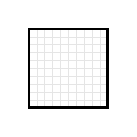
\begin{tikzpicture}[yscale=-1,
				mill/.style={line width=.1mm,gray!20},
				cent/.style={thick,gray!60}]
			\begin{scope}
				\clip (0,0) rectangle (\WW,\HH);
				\foreach \i in {1,...,180}
				\draw[mill] (\i*0.1,0) -- (\i*0.1,\HH);
				\foreach \i in {1,...,270}
				\draw[mill] (0,\i*0.1) -- (\WW,\i*0.1);
				\foreach \i in {1,...,18}
				\draw[cent] (\i,0) -- (\i,\HH);
				\foreach \i in {1,...,27}
				\draw[cent] (0,\i) -- (\WW,\i);
			\end{scope}
			\draw[line width=1pt] (0,0) rectangle (\WW,\HH);
		\end{tikzpicture}

	}
\end{document}
